\documentclass[12pt]{article}
\usepackage[margin=1in]{geometry}
\usepackage[protrusion=true,
            expansion=true]{microtype}
%\usepackage{amssymb}
%\usepackage{amsmath}
\usepackage{booktabs}
\usepackage{color}
\usepackage[usenames,
            dvipsnames]{xcolor}
\usepackage{graphicx}
\usepackage{caption}
\usepackage{subcaption}
\usepackage{algorithm}
\usepackage{algorithmic}

\usepackage{kpfonts}
\usepackage[T1]{fontenc}
\usepackage{setspace}
\singlespacing
%\onehalfspacing
%\doublespacing

\newcommand{\term}[1]{\emph{#1}}

\begin{document}

\title{Programs that Program}

\author{Keenan Breik, Jason Liang}
\date{}
\maketitle

\begin{abstract}
To use evolutionary computation
to solve problems effectively and efficiently,
we need good incarnations.
Many hand-designed schemes exist,
but although such schemes have been selected or tuned
using evolutionary computation,
we suspect this is too limiting.
%they have not been \emph{created}
%using evolutionary computation.
By evolving a population
that guides its own evolution,
we can escape hand-design.
To take a step toward doing so,
we present a way of evolving neural networks
that generate other neural networks.
%This can form the foundation
%for later developing
%a full, automatically designed and optimized
%scheme for evolutionary computation.
We present techniques for evolving
neural networks that generate other neural networks.
We find that they work
but that the networks produced
can have pathological or trivial structure.
%but we can get better results
%but instead evoling schemes.
\end{abstract}

\section{Introduction}
\label{intro}

Evolutionary computation allows computers
to automatically solve problems
that can be cast as optimization problems.
Until now, implementations have been
in large part hand designed.
Designers struggle to find meaningful constructs
and optimal tunings that allow evolutionary computation
to efficiently and effectively solve problems.
%to efficient, effective evolutionary computation.
%This design is part of solving target problems,
But once it is factored into the cost
of solving that problem,
that struggle is unjustifiable.

We propose to allow computers
to automatically design such implementations
by using evolutionary computation itself.
One way of doing this is to set up
an existing implementation,
such as genetic programming,
to search for a better one.
But by using a fixed implementation,
we must wait until the the process completes
to get a usable result,
and we still must hand-pick that fixed implementation.
An alternative is to start with an implementation
and allow it to modify itself.
Thus it would improve over time
and also improve at improving itself.

Two essential elements of an implementation
that must be established
are the candidate solution representation
and the population operators.
The representation is a form for storing a candidate
along with a decoding method
to extract it from storage.
To be general,
this representation can be an arbitrary program.
The population operators
generate new individuals from the current population.
To be general,
these operators can be arbitrary programs.

In this paper,
we demonstrate that neural networks
can generate other meaningful neural networks.
Since arbitrary neural networks are computationally powerful,%
\cite{sperduti1997netpower}
we can use them as candidate solution representations
and also as population operators.
Here however,
as a first step,
we only evolve networks
that generate sensible networks
or that generate themselves.

%[explain how programs that program
%would give us this]
%
%To do so, we desire programs
%that write other programs
%and thereby explore a search space.
%
%In this paper,
%we demonstrate that neural networks
%can generate other meaningful neural networks.
%[Be clear. Elaborate.]

%[Explain why self-replication.]

The following is an overview of the rest of the paper.
In section \ref{problemstatement},
we discuss the general problem of generating networks.
In section \ref{feedforward},
we go over our methods
for constructing self-replicating feedforward neural networks.
In section~\ref{arbitrary},
we discuss our methods
for constructing replicating arbitrarily recurrent
neural networks.
In section \ref{results},
we discuss experimental results.
Finally in section \ref{conclusion},
we present conclusions and future work.

\section{Related Work}
\label{related}

Evolutionary computation
has many incarnations
and has been used to solve a wide variety of problems.
%\cite{angeline1994evolutionary}
It has been used in general to optimize parameters
\cite{back1993overview}
and has been used to solve numerous engineering problems
\cite{dasgupta1997evolutionary},
such as designing mission-critical attennas for NASA
\cite{hornby2006automated}.
It has also been useful
even when numerous criteria must be satisfied
\cite{fonseca1995overview}.

In a thread more similar to our work,
evolutionary computation has been used
to tune existing implementations
of evolutionary computation
in a process dubbed meta-optimization
\cite{brest2006param}.
These implementations
have parameters that must be selected,
and selecting them optimally by hand is difficult
and can be time consuming.

So-called hyper-heuristics
have been used to avoid choosing a single fixed implementation
\cite{burke2010classification},
and parameter-free, self-optimizing metaheuristics
have also been used to avoid
manual tuning \cite{brest2006param}.
But both of these are limited
to manipulating existing implementations
of evolutionary computation.

Evolutionary computation
has also been used to program computers automatically
\cite{koza1999genetic}.
We are also interested in programming computers automatically,
but we are not interested so much
in producing programs
for solving particular problems
as we are in producing programs
that produce other programs
(possibly \textit{ad infinitum}).

%Gentic programming has been used
%to automatically develop computer programs.
%Evolutionary
To produce programs that program,
we draw on the notion of a CPPN (compositional
pattern-producing network).\cite{stanley2007cppn}
CPPNs, however, are meant to encode the structure
of a network, whereas we use corruptions of them
for more general purpose information storage
and pattern generation.

%Genetic programming?
%Compositional pattern-producing networks.

\section{Decoding Networks}
\label{problemstatement}

A feedforward neural network $N$ encodes a function $f_N$
and thus is capable of storing information.
An arbitrary neural network $N$ encodes a program $P_N$
and thus is also capable of storing information.
One type of information a network may store
is an encoding of a second neural network $D(N)$.
But just as the meaning of a word
depends on the language being spoken,
so does the network encoded by $N$
depend on the semantics chosen.

To establish these semantics,
we may define what $N$ should be
in order to encode a given network $D(N)$.
This is the problem of \term{encoding}.
But if we want a network $N$
to generate another network $D(N)$,
then $D(N)$ is not given.
It is generated.
Solving the problem of encoding does not help.

An alternative way to establish the semantics
is to define what network $D(N)$ is encoded
by a given network $N$.
This is the problem of \term{decoding},
and we focus on it.
Solving the problem of decoding
consists of defining $D$
and allows us to have neural networks
generate other neural networks.

In order to give a network $N$
the power to generate another network
in an interesting way,
we prefer the decoding function $D$
to be neither completely stable
nor completely chaotic.
Instead, we want it somewhere around the edge of chaos.%
\cite{langton1990edgechaos}%
\cite{bertschinger2004edgechaos}
This seems to pose a challenge,
but the function or program a neural network encodes
satisfies exactly this property.
So we can define $D(N)$ in terms of $f_N$ or $P_N$.
In other words, part of computing $D(N)$
can be applying $f_N$ or $P_N$.

We can consider the features of $D(N)$,
such as how its neurons connect,
to be stored at particular points
in $f_N$
or to be outputs of $P_N$.
To extract the features of $D(N)$,
we simply query $N$ at such points.

%We consider ? schemes.
%[x0 ... xn] [y0 ... yn] ---> w
%[L S t s] ---> [n n w]
%arbitrary network

%\section{Evolution}
%algorithms. fitness functions.

\section{Self-replicating Feedforward Networks}
\label{feedforward}

To create a self-replicating feedforward neural network,
we first use the pyBrain neural network library \cite{schaul2010}
to create an initial neural network that has a fixed topology.
By fixed topology, we mean that
the number of input neurons,
output neurons,
hidden layers,
neurons, and number of connections remain constant.
The only parameters we plan to optimize
in order to generate self-replicating neural networks
are the weights of the connections between neurons.
Since a feedforward neural network
can have many variations in its topology,
we have chosen a simple structure that makes the most sense.

One major challenge is deciding what kind of input
to feed into the neural network and how to interpret the output
of the neural network as another neural net.
For simplicity,
we decided on giving our neural network a N-bit vector
of binary numbers as input.
If we sequence all the connections in the neural network,
we can associate the value of binary vector
with a corresponding connection.
For example, the binary vector 1001
can be associated with the 5th connection
in a small network with 8 connections in total.
Accordingly, the output of the neural network
is a single value
and it represents the weight
of the connection specified by the input vector.
Thus by feeding the neural network
a set of inputs that map to all the connections in the network,
we can generate weights for each of connections.
This means that the network is capable of generating another net
exactly like itself in topology,
but with possibly different connection weights. 

\begin{figure}[h]
\begin{center}
  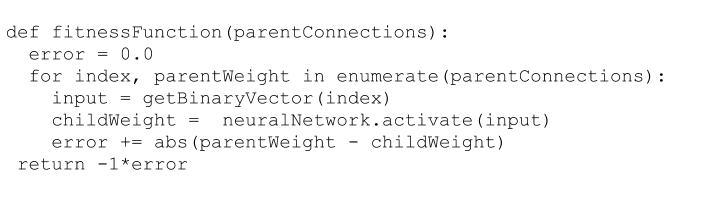
\includegraphics[width=0.8\linewidth]{pseudo.png}
\end{center}
   \caption{Function for computing fitness of a neural network.
For each connection in the parent network,
we convert it into a binary vector,
feed it as input,
and get the connection weight
of the same connection in the child network.
We compare the difference
between the child and parent weights
and sum up all differences as error,
which is then inverted to become a fitness value.}
\label{pseudo}
\end{figure} 

The next step is to come up with
a method to optimize the connection weights
of the original network such that child network generated
also has the same connection weight.
Given the lack of gradients in this problem,
we decide to rely on a black-box optimization approach
to optimize the connection weights of the parent network.
Thus we require a fitness function
that evaluates how close the neural network is
to generating a child network exactly like itself.
To compute a fitness value,
as seen in Fig.~\ref{pseudo},
we use the parent network
to compute the connection weights of the child network,
determine the error between the new connection weight
and its original value in the parent network,
and return the sum of all the errors.
We try a variety of different black-box optimization methods,
including genetic algorithms \cite{deb2002fast},
CMA-ES \cite{hansen2003reducing},
and NES \cite{wierstra2008natural}
to try to minimize the error
and maximize the fitness of the neural network.

\section{Replicating Arbitrary Networks}
\label{arbitrary}

We also worked with arbitrarily recurrent neural networks.
Again we are faced with the problem
of specifying inputs and outputs.
One option is to do so in the same way
as with feedforward neural networks.
%as summarized in figure~\ref{arbitrarybadio}.
But since we will need
to repeatedly halt the network
after some arbitrary interval
and restart it,
this approach does not exploit
the power of recurrency.
%But since recurrent neural networks
%have no natural point of completion,
%we must halt them
%But this requires running the network
%But this does not exploit
So instead we allow the network to run freely
and output at its own pace.

We use a sigmoidal activation function $a$ onto $[0, 1]$.
%We use the activation function $a : \mathbb{R} \to [0, 1]$
%defined by $a(x) = 1 / exp$
Because of the distortion
that bounded activation functions introduce,
treating or interpreting an input or output
as an unbounded signal
can make large parts of its range unuseable.
So we treat each output
as a single bit.
As summarized in figure~\ref{arbitraryio},
we allocate several bits
to each output number,
and we reconstruct it from the bit string
$B = b_0...b_n$
as $N(B) = \sum \operatorname{round}(b_0) \cdot 2^0$.
To recover the weight we compute $\tan(m \cdot N(B) - b)$
where $m$ and $b$ are chosen so that $m \cdot N(B) - b$
always lies in some subset of a single period of $\tan$.
This allows weights a wide range
while retaining fine granularity near 0.

Notice that we specify no inputs.
This is because the neural network is taken to be a program
that will output another neural network
as a sequence of connections.
Each output tuple $(r, t, s, w_{t\,s})$
is interpreted as a connection to $t$ from $s$
with weight $w_{t\,s}$ if and only if $r$ is on.
Since the halting problem is not computable,
there is no way to know
when the last connection has been output.
To cope with this
we define $C_\text{max}$ to be 65536
and halt the network after it has run
for $C_\text{max}$ steps.

%So input
%each input and output should be interpreted as discrete
%rather than 
%Due to the distortive nature of bounded activation functions,

%\begin{figure}[h]
%  \centering
%  \begin{tabular}{@{}ll@{}}
%  \toprule
%  inputs             & outputs \\
%  \midrule
%  neuron count flag  & neuron count \\
%  target neuron, $t$ & weight $w_{t \, s}$ \\
%  source neuron, $s$ & \\
%  \bottomrule
%  \end{tabular}
%  \caption{}
%  \label{arbitrarybadio}
%\end{figure}

\begin{figure}[ht]
  \begin{minipage}[b]{0.45\linewidth}
  \centering
  %\begin{figure}[h]
    %\centering
    \begin{tabular}{@{}llll@{}}
    \toprule
    inputs             &           & outputs & \\
    \cmidrule(rl{0em}){1-2}          \cmidrule(rl{0em}){3-4}
                       & bits      &         & bits \\
    \midrule
                       &           & ready signal, $r$     & 1 \\
                       &           & target neuron, $t$   & 8 \\
                       &           & source neuron, $s$   & 8 \\
                       &           & weight, $w_{t \, s}$ & 8 \\
    \bottomrule
    \end{tabular}
  %\end{figure}
  \end{minipage}
  %
  \hspace{\fill}
  %
  \begin{minipage}[b]{0.45\linewidth}
    \centering
    \begin{tabular}{@{}llll@{}}
    \toprule
    inputs             &           & outputs & \\
    \cmidrule(rl{0em}){1-2}          \cmidrule(rl{0em}){3-4}
                       & bits      &         & bits \\
    \midrule
                       &           & ready signal, $r$    & 1 \\
    task input, $x$    & 1         & task output, $o$     & 1 \\
    task input, $y$    & 1         &                      &   \\
                       &           & target neuron, $t$   & 8 \\
                       &           & source neuron, $s$   & 8 \\
                       &           & weight, $w_{t \, s}$ & 8 \\
    \bottomrule
    \end{tabular}
  \end{minipage}
  \caption{Inputs and outputs used
    (left) in the original simple scheme
    and (right) with a task that eases
    computing the fitness function.}
  \label{arbitraryio}
\end{figure}


To evolve these networks we again use NEAT.
Since we are trying to evolve replication,
we choose a fitness function that does so directly.
We decode the network repeatedly
until the result is no longer sensible
and reward it for more decodings.
This however presents two problems:
it is difficult to judge when a network is not sensible
and this fitness is discrete and so has a weak gradient.

To address this we introduce a task,
as summarized in figure~\ref{arbitraryio}.
The task need not be (and perhaps should not be)
difficult.
It need only give us a way
of weeding out networks that are not sensible.
In our experiments,
the task was computing logical or.
To judge the fitness of a network $N$,
we repeatedly evaluate $N$ at the task
and then decode it to get $D(N)$
and do the same with $D(N)$.
This is summarized in figure~\ref{fitalg}.

\begin{figure}[h]
  \centering
  %\begin{algorithm}
  %\par
  \begin{minipage}[c]{.5\textwidth}
  \begin{algorithmic}
  \STATE $f \leftarrow 0$
  \LOOP
  \STATE $f' \leftarrow$ performance of \textit{net} at task
  \IF{$f'$ does not exceed a threshold}
  \RETURN $f$
  \ENDIF
  \STATE $f \leftarrow f + f'$
  \STATE \textit{net} $\leftarrow$
    $\operatorname{decode}(\textit{net})$
  \ENDLOOP
  \end{algorithmic}
  %\end{algorithm}
  \caption{Determining the total fitness
    of a neural network \textit{net}.}
  \label{fitalg}
  \end{minipage}
\end{figure}

%\begin{figure}[h]
%  \centering
%  \caption{}
%  \label{arbitrarybetterio}
%\end{figure}


%To evaluate the fitness of a ne
%In this setup however

We tried several other cursory approaches that failed,
and so carefully developed this approach.
At the time of this publishing, however,
we have not successfully run our experiments.

\section{Experimental Results}
\label{results}

In an experiment, we test to see if feedforward neural networks
could replicate themselves using the method described
in section \ref{feedforward}.
For our feedforward neural network topology,
we decide on having an input layer with 8 neurons,
2 hidden layers with 12 neurons each,
and finally an output layer with a single neuron.
This network structure seems to have a good balance
between complexity, number of inputs, and performance.
All layers are fully connected
and each neuron uses a sigmoid
as its activation function.
The sigmoid allows the neural network
to output any range of values between -1 and 1.
Accordingly, the connection weights
of all the neurons are all randomly initialized between -1 and 1.
Experimentally, out of all the black box optimization methods, 
we found that using CMA-ES resulted in the most improvement 
in fitness every generation. Thus, we optimize using CMA-ES
as described in the methodology for 500 generations.

Fig.~\ref{result1} shows how error goes down
as a function of the number of generations
that black-box optimization is applied
to connection weights of the parent network.
As we can see by the blue curve,
the error starts off around 150 and smoothly converges
to a value of around 5 at the 500th generation mark.
To show that our optimization method
and fitness functions are robust,
we deliberately clamp a certain percentage
of the connection weights (10\%, 20\%, and 40\%),
which results in the other curves
shown in Fig.~\ref{result1}.
While the final errors are not as good
as when none of the weights are clamped,
significant reductions in errors are still present.

However, while optimizing the connections
of the parent network results in a child network
that is similar to the parent,
the connection weights themselves do not seem
to be very interesting.
Fig.~\ref{histogram}(a) and (b) shows a histogram
of the connection weights
of both the optimized parent network
and the resulting child network respectively.
As we can see, the connections in both networks
have roughly the same weights
at around roughly the 0.10 to 0.15 range.
From this, we can conclude that
if all the weights in a neural network are roughly the same,
the output of the neural network are also in the same range,
no matter what kind of input is given.
Thus the question arises whether it is
possible to create self-replicating networks
where the weights have interesting distributions. 

\begin{figure}[h]
\begin{center}
  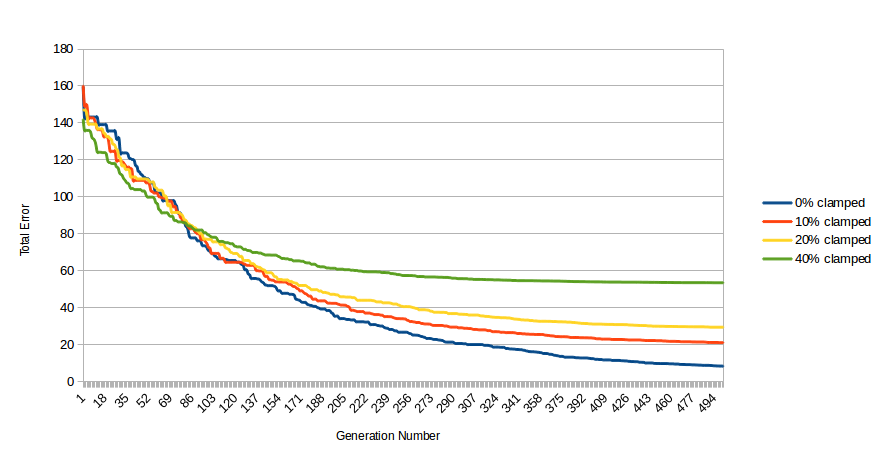
\includegraphics[width=1.0\linewidth]{result1.png}
\end{center}
   \caption{This chart shows error (as defined in section \ref{feedforward}) as a function of number of generations. The legend shows the percentage of connections that are clamped (fixed so that they do not change).}
\label{result1}
\end{figure}

\begin{figure}[h]
\begin{center}
  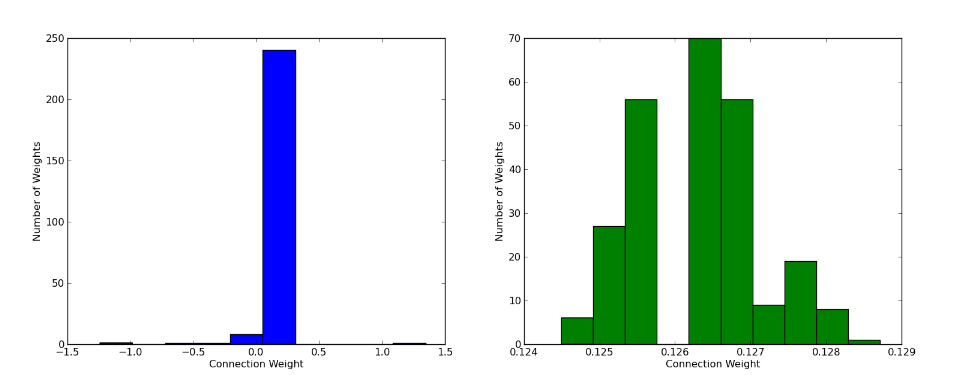
\includegraphics[width=1.0\linewidth]{histogram.png}
\end{center}
   \caption{(a) Histogram of weights of parent network after optimization. (b) Histogram of weights of child network that result from parent network.}
\label{histogram}
\end{figure}

\section{Conclusion and Future Work.}
\label{conclusion}

In this project, we demonstrate that it is possible to generate
a feed-forward neural network that when given a series of nonrandom inputs,
output the weights of another child network which also
have roughly the same connection weights. Unfortunately, both the
child and parent networks are uninteresting in that the weights are all roughly
the same value. A major question that remains is whether self replicating neural 
networks with unique and interesting weight distributions can be generated.

Given our experiments with neural networks, we strongly suspect that this is
not possible with just a fully connected feed-forward structure. Instead, we believe
that it might be possible to incrementally build up a neural network with arbitrary
complex topology using NEAT \cite{stanley2004efficient} that capable is of outputting
its own topology and weights when given an ordered, logical set of inputs. 
For future work, we plan to use NEAT with a fitness 
function such as the one used for feed-forward neural networks to create self-replicating
neural networks. However, we also strongly
suspect that the fitness landscape for this type of problem is highly deceptive.
Therefore, we will also like to try using novelty search \cite{lehman2008exploiting}
instead of a conventional fitness function.

Finally, another important issue is whether these self-replicating networks
can be used to do useful work. We hypothesize that these kind of networks exhibit
behavior that are on the ``edge of chaos" and thus have maximized their potential
to do computation. Thus, we plan to explore whether the structure of
self-replicating networks allow them to be easily tuned towards certain tasks, such as digit
recognition or object classification.

\renewcommand{\refname}{\section{References}}
\bibliography{selfrep}
\bibliographystyle{plain}

\end{document}
